% !BIB TS-program = biber
% !TeX TS-program = xelatex
% ================ %
%      导言区      %
% ================ %
\documentclass[usenames,dvipsnames,svgnames,xcolor = table]{beamer}
\usetheme[ColorDisplay=BSblue, ContentMuticols=ture]{nudt}
% \addbibresource[location=local]{refs/ref.bib}
% \special{dvipdfmx:config z 0} %取消PDF压缩,加快速度,最终版本生成的时候最好把这句话注释掉
% Add option 'aspectratio=169' for 16:9 widescreen 
% Add option  'handout' to ignore animations
% --------title page-------- %
\title[国防科技大学 | 高等数理统计习题课]{\LARGE 高等数理统计习题课}
\subtitle{第三组} % subtitle 未设置页脚显示项, 请在 title 中设置.
\author[张鑫航]{
    汇报人:\href{mailto:zhangxinhang19@foxmail.com}{张鑫航}\\
    \medskip
    数学
}
\institute{国防科技大学}
\date{\today}
% ------正文区------ %
\begin{document}

% --------总目录-------- %
% 可注释.
\begin{frame}{目录}
    \begin{multicols}{2}
        \large{
        \tableofcontents
        }%
      \end{multicols}
\end{frame}

% --------节: 声明------------ % 

\section{基本概念}
\subsection{统计结构}
\begin{example}
    对一物理量进行测量,其真值$\mu$未知,测量值为$x$,但测量有误差,故可认为
    \[
        x = \mu+\varepsilon
    \]
    $\{ x_1,x_2\cdots,x_n \}$是测量值。

    可加上一个假设,进一步设$\varepsilon\sim N(0, \sigma^2)$,这就建立了一个\textbf{\textcolor{main1}{统计结构}}。
\end{example}
\begin{definition}[统计结构]
    设$(\mathscr{X},\mathscr{B})$为一可测空间,$\mathscr{P}$为其上的一族概率分布,则成三元组$(\mathscr{X},\mathscr{B},\mathscr{P})$为统计结构(模型)。若$\mathscr{P}$仅依赖于某参数(向量)$\theta$,即$\mathscr{P} = \{ \mathscr{P}_{\theta}:\theta\in \Theta \}$,就称为参数结构,否则成为非参数结构。
\end{definition}

\begin{definition}[乘积结构与重复抽样结构]
    设$(\mathscr{X},\mathscr{B},\mathscr{P})$与$(\mathscr{X}',\mathscr{B}',\mathscr{P}')$为两个统计结构,则称$(\mathscr{X}\otimes \mathscr{X}',\mathscr{B}\otimes \mathscr{B}',\mathscr{P}\otimes \mathscr{P}')$为二者的乘积结构,记为$(\mathscr{X},\mathscr{B},\mathscr{P})\otimes (\mathscr{X}',\mathscr{B}',\mathscr{P}')$,特别的,$n$个同样的统计结构的乘积称为重复抽样结构,记为$(\mathscr{X},\mathscr{B},\mathcal{P})^{n}$或$(\mathscr{X}^{n},\mathscr{B}^{n},\mathcal{P}^{n})$。
\end{definition}

\begin{definition}[样本分布函数]
    设$ (\mathscr{X},\mathscr{B},\mathscr{P})^{n} $为一重复抽样结构,$\forall (X_1, X_2, \cdots, X_n)\in X^n$,定义
    \[
        F_n(x) = \dfrac{1}{n}\sum\limits_{i = 1}^{n}I_{(X_i\leqslant x)}
    \]
    为经验分布函数(\textcolor{thid1}{样本分布函数})。
\end{definition}

\begin{definition}[所控]
    设$u$和$v$是可测空间上$(\mathscr{X},\mathscr{B})$上的两个\textcolor{main1}{$\sigma$-有限测度}。若$N\in \mathscr{B}, \ u(N) = 0\Rightarrow v(N)=0$,则称\textcolor{thid1}{$v$关于$u$绝对连续},或$v$被$u$所控,记为$v<<u$。
\end{definition}

\begin{definition}[可控结构]
    设$(\mathscr{X},\mathscr{B},\mathscr{P})$为一统计结构,若存在$u$为可测空间$(\mathscr{X},\mathscr{B})$上的$\sigma-$有限测度,使得$\forall P\in \mathscr{P},\ P<<u$,则称该结构为\textcolor{thid1}{可控结构}。进而$p(x) = \dfrac{dP(x)}{du}$成为p.r密度。
\end{definition}

\subsection{常用分布族}
\subsubsection{Gamma分布族}
\begin{definition}[Gamma分布族]
    在$(R^+, \mathscr{B}_{R^+})$上的密度函数形如
    \[
        p(x;\alpha, \lambda) = \dfrac{\lambda^\alpha}{\Gamma(\alpha)}x^{\alpha-1}e^{-\lambda x}I_{(0,+\infty)}(x),\ (\alpha>0, \lambda>0)  
    \]
    的分布称为参数为$\alpha,\ \lambda$的\textcolor{main1}{Gamma分布族},记为$Ga(\alpha, \lambda)$。其中,$\Gamma(\alpha) = \int_{0}^{+\infty}x^{\alpha-1}e^{-x}\ dx$为Gamma函数。
\end{definition}

\begin{note}
    因为$\int_{0}^{+\infty}\lambda^\alpha x^{\alpha-1}e^{-\lambda x}\ dx= \int_{0}^{+\infty} (\lambda x)^{\alpha-1}e^{-\lambda x}\ d(\lambda x) = \Gamma(\alpha)$,所以,
    \[
        \int_{-\infty}^{+\infty} p(x;\alpha, \lambda) = \dfrac{\Gamma(\alpha)}{\Gamma(\alpha)} = 1
    \]
\end{note}

\begin{note}
    \begin{itemize}
        \item 由图~\ref{fig:gamma},$\alpha$影响$Ga(\alpha, \lambda)$的形状,$\lambda$影响$Ga(\alpha, \lambda)$的尺寸
        \item $\alpha\leqslant 1$时,严减;$1<\alpha\leqslant 2$时,先上凸,后下凸;$\alpha>2$时,先下凸,再上凸,最后下凸,两个拐点
        \item $\lambda$影响密度函数的胖瘦
    \end{itemize}
\end{note}

\begin{figure}[htbp]
    \centering
    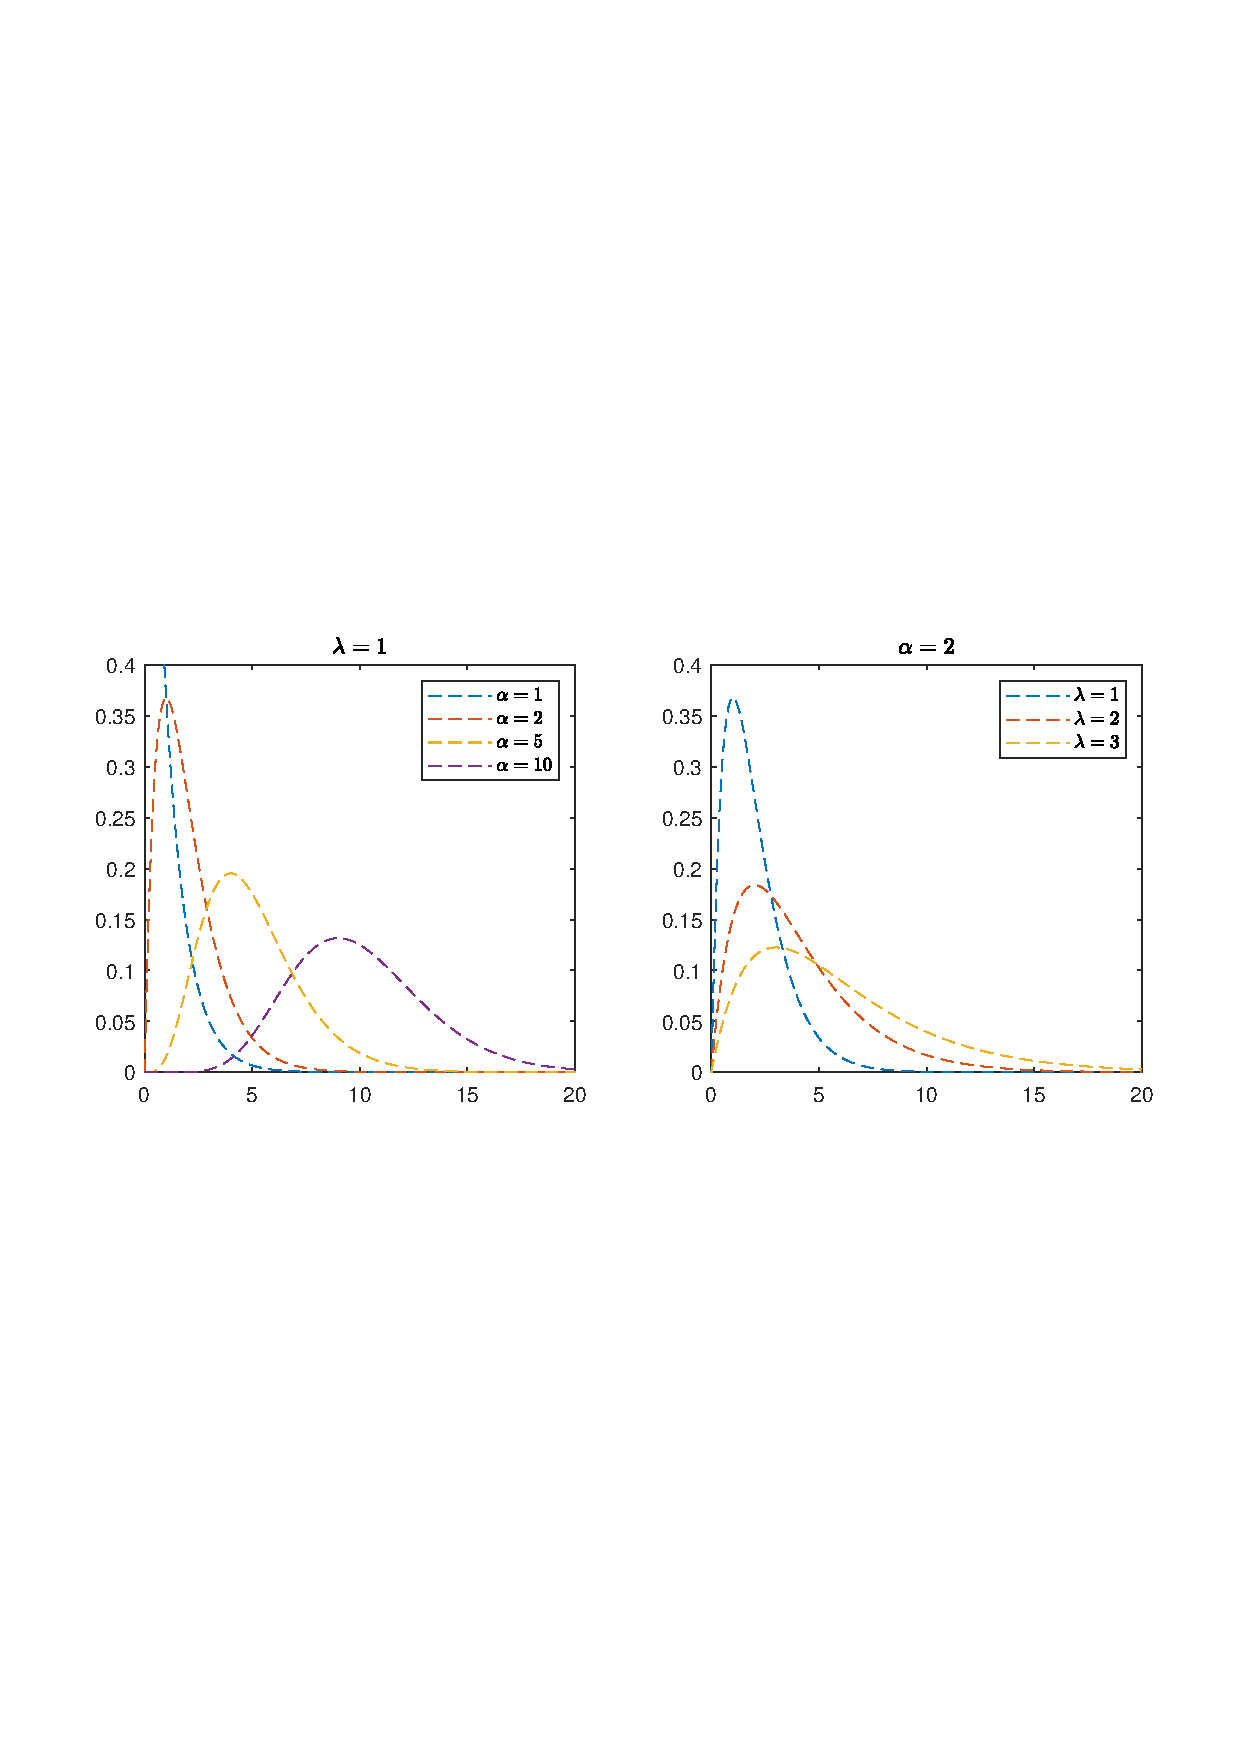
\includegraphics[width =.7\textwidth]{image/gamma.pdf}
    \caption{$\alpha$和$\lambda$对$Ga(\alpha, \lambda)$的影响}
    \label{fig:gamma}
\end{figure}

设$Z\sim Ga(\alpha, \lambda)$,则其$k$阶矩
\[
    \begin{array}{ll}
        EZ^{k}& = \displaystyle\int_{0}^{+\infty} \dfrac{\lambda^\alpha}{\Gamma(\alpha)}x^{\alpha+k-1}e^{-\lambda x}\ dx \\
        & = \dfrac{\Gamma(\alpha+k)}{\Gamma(\alpha)\lambda^k}\displaystyle\int_{0}^{+\infty} \dfrac{\lambda^{\alpha + k}}{\Gamma(\alpha+k)}x^{\alpha+k-1}e^{-\lambda x}\ dx \\
        &=\dfrac{\Gamma(\alpha+k)}{\Gamma(\alpha)\lambda^k} = \dfrac{(\alpha+k-1)(\alpha+k-2)\cdots \alpha}{\lambda^k}
    \end{array}
\]

$Ga(\alpha, \lambda)$的\textcolor{thid1}{特征函数}
\[
    \begin{aligned}
        f(t)& =Ee^{ixt}=\int_{0}^{+\infty}\frac{\lambda^{\alpha}}{\Gamma(\alpha)}x^{\alpha-1}e^{-\lambda(1-\frac{it}{\lambda})x}dx  \\
        &=(1-\frac{it}{\lambda})^{-\alpha}\int_{0}^{+\infty}\frac{\lambda^{\alpha}}{\Gamma(\alpha)}[(1-\frac{it}{\lambda})x]^{\alpha-1}e^{-\lambda(1-\frac{it}{\lambda})x}d(1-\frac{it}{\lambda})x \\
        &=(1-\frac{it}{\lambda})^{-\alpha}
    \end{aligned}
\]
于是,设$Z_1,Z_2,\cdots,Z_n\sim Ga(\alpha, \lambda)$,且$Z_i$相互独立,则
\[
    Z_1+Z_2+\cdots+Z_n\sim Ga(\alpha_1+\alpha_2+\cdots+\alpha_n,\lambda)
\]

两个\textcolor{main1}{特殊的Gamma分布}
\begin{itemize}
    \item 1) $Ga(1, \lambda) = Exp(\lambda),\ p(x,\lambda) =\lambda e^{-\lambda x}$
    \item 2) $Ga(\frac{n}{2},\frac{1}{2})=\chi^2(n),\quad p(x,n)=\dfrac{1}{2^{n/2}\Gamma(n/2)}x^{n/2-1}e^{-x/2},x>0$
\end{itemize}
\begin{note}
    $Z \sim \chi^2(n)$,则
    \[
        \begin{array}{l}
            EZ = \dfrac{n/2}{1/2} = n\\
            EZ^2 = \dfrac{(n/2+1)(n/2)}{(1/2)^2}=n^2+2n \\
            VarZ = EZ^2-(EZ)^2 = 2n
        \end{array}   
    \]
\end{note}
\begin{example}
    电子产品的失效常常是由于外界的“冲击”引起。若在$(0,t)$内发生冲击的次数$N(t)$服从参数为$\lambda t$的泊松分布,试证明第$n$冲击到来的时间服从伽马分布$Ga(n,\lambda)$
\end{example}
\begin{proof}
    \[
        \begin{array}{c}
            \{ S_n\leqslant t\} = \{ N(t)\geqslant n\}\\
            F_{S_{n}(t)} = P\{S_n\leqslant t\} = P\{ N(t)\geqslant n\} = \sum\limits_{k =n}^{\infty}\dfrac{(\lambda t)^{k}}{k!}e^{-\lambda t}\\
            F_{Ga(n,\lambda)}(t) = \displaystyle\int_{0}^{t}\dfrac{\lambda^n}{\Gamma(n)}x^{n-1}e^{-\lambda x}\ dx \overset{?}{=} 1-\sum_{k=0}^{n-1}\frac{(\lambda t)^{k}}{k!}e^{-\lambda t}=\sum_{k=n}^{\infty}\frac{(\lambda t)^{k}}{k!}\mathrm{e}^{-\lambda t}
        \end{array}
    \]
\end{proof}

\subsubsection{Beta分布族}
\begin{definition}[Beta分布]
    设$D=(0,1)$,定义在$(D,\mathscr{B}_D)$,密度函数形如$p(x;a,b) = \dfrac{1}{B(a,b)}x^{\alpha-1}(1-x)^{b-1}I_{(0,1)}(x),\ (a>0, b>0)$的分布成为参数为$a,\ b$的Beta分布,记为$Be(a,b)$。其中$B(a,b) = \displaystyle \int_{0}^{1}x^{a-1}(1-x)^{b-1}\ dx = \dfrac{\Gamma(a)\Gamma(b)}{\Gamma(a+b)}$    
\end{definition}

\begin{itemize}
    \item $a>1$和$b>1$,$p(x)$单峰状,在$x = (a-1)/(a+b-2)$处达到最大值
    \item $a<1$和$b<1$,$p(x)$U形,在$x = (a-1)/(a+b-2)$处达到最小值
    \item 当$a = b+1/2$时,Beta分布为反正弦分布
    \item $a<1$和$b>1$,$p(x)$严减
    \item $a>1$和$b<1$,$p(x)$严增
\end{itemize}

\begin{note}
    设$Z\sim Be(a, b)$,则$Z$的$k$阶矩
    \[
        \begin{array}{ll}
            EZ^k &= \displaystyle\int_{0}^{1}\dfrac{1}{B(a,b)}x^{a+k-1}(1-x)^{b-1}\ dx\\
            &=\dfrac{B(a+k,b)}{B(a,b)}\displaystyle\int_{0}^{1}\dfrac{1}{B(a+k,1)}x^{a+k-1}(1-x)^{b-1}\ dx\\
            &= \dfrac{B(a+k,b)}{B(a,b)} = \dfrac{\Gamma(a+k)\Gamma(b)}{\Gamma(a+k+b)}\cdot \dfrac{\Gamma(a+b)}{\Gamma(a)\Gamma(b)}=\dfrac{\Gamma(a+k)\Gamma(a+b)}{\Gamma(a)\Gamma(a+k+b)}\\
            &=\dfrac{(a+k-1)(a+k-2)\cdots (a)}{(a+b+k-1)(a+b+k-2)\cdots (a+b)}
        \end{array}
    \]
    特别的,
    \[
        \operatorname{E}Z = \dfrac{a}{a+b},\quad \operatorname{E}Z^2 = \dfrac{(a+1)a}{(a+b+1)(a+b)} ,\quad  \operatorname{Var}Z = \operatorname{E}Z^2-(\operatorname{E}Z)^2=\left[ (\dfrac{a+1}{a+b+1})^2-1 \right](\dfrac{a}{a+b})^2
    \]
\end{note}

\textcolor{red}{Beta分布与Gamma分布的关系}

设$X_1\sim \Gamma(\alpha_1, \lambda),\ X_2\sim \Gamma(\alpha, \lambda)$,且相互独立,则$Y = \dfrac{X_1}{X_1+X_2}\sim Be(\alpha_1, \alpha_2)$
\begin{proof}
    $X_1$和$X_2$的联合分布为
    \[
        p_{X_1,X_2}(x_1,x_2) = \dfrac{\lambda^{\alpha_1 + \alpha_2}}{\Gamma(\alpha_1)\Gamma(\alpha_2)}x_{1}^{\alpha_1-1}e^{-\lambda x_1}x_{2}^{\alpha_2-1}e^{-\lambda x_2}
    \]
    令$U= X_1,\ V = \dfrac{X_1}{X_1+  X_2}$,则$\left\{\begin{array}{l}
        X_1 = U\\
        X_2 = U/V-U
    \end{array}\right.$,且变换的行列式为
    \[
        \left\lvert \begin{matrix}
            1 & 0\\
            1/v-1& -u/v^2
        \end{matrix}\right\rvert 
    \]
    $U,V$的联合分布为
    \[
        \begin{array}{ll}
            p_{U,V}(u,v) &= p_{X_1,X_2}(u,v)|J|\\
            &=\dfrac{\lambda^{\alpha_1+\alpha_2}}{\Gamma(\alpha_1)\Gamma(\alpha_2)}u^{\alpha_1-1}e^{-\lambda u}(\frac{u}{v}-u)^{\alpha_2-1}e^{-\lambda(u/v-u)}\frac{u}{v^2}
        \end{array}
    \]
    则$V$的边缘分布为
    \[
        p_{V}(v) = \displaystyle\int_{0}^{\infty} p_{U, V}(u,v)\ du =\dfrac{\Gamma(\alpha_1+\alpha_2)}{\Gamma(\alpha_1)\Gamma(\alpha_2)}v^{\alpha_1-1}(1-v)^{\alpha_2-1}
    \]
    即$Y_2\sim Be(\alpha_1, \alpha_2)$
\end{proof}

\textcolor{red}{Beta-Binomial共轭性}
\begin{proof}
    假定二项分布$b(n,p)$的参数$p$服从$Be(a,b)$的先验分布。然后又做了$n_1+n_2$次伯努利试验(记为$W$)成功$n_1$次,失败$n_2$次,于是后验分布
    \[
        \begin{array}{l}
            P(p|W) = \dfrac{P(p,W)}{P(W)} = \dfrac{P(W|p)P(p)}{\int_{0}^{1}P(W|p)P(p)dp}\\
            \dfrac{C_{n_1+n_2}^{n_1}p^{n_1}(1-p)^{n_2}\frac{1}{B(a,b)}p^{a-1}(1-p)^{b-1}}{\int_{0}^{1}C_{n_1+n_2}^{n_1}p^{n_1}(1-p)^{n_2}\frac{1}{B(a,b)}p^{a-1}(1-p)^{b-1}\ dp}=\dfrac{p^{n_1+a-1}(1-p)^{n_2+b-1}}{\int_{0}^{1}p^{n_1+a-1}(1-p)^{n_2+b-1}\ dp}\\
            = \dfrac{p^{n_1+a-1}(1-p)^{n_2+b-1}}{B(n_1+a-1,n_2+b-1)}
        \end{array}
    \]
    $p$的后验分布为$Be(n_1+a, n_2+b)$,$Be(a,b) + \mathrm{BinomCount}(n_1, n_2) = Be(n_1 + a, n_2 + b)$。
\end{proof}

\subsubsection{Fisher分布族}

\begin{definition}[Fisher Z分布]
    定义在$(R^+,\mathscr{B}_{R^+})$上的密度函数形如
    \[
        p(x;a,b) = \dfrac{1}{B(a,b)}\dfrac{x^{a-1}}{(1+x)^{a+b}}I_{(0,+\infty)}(x),\ (a>0,b>0)
    \]
    的分布承诺为参数为$a,b$的Fisher Z分布,记作$Z(a,b)$。
\end{definition}
设$Z\sim Z(a,b)$,则$Z$的$k$阶矩
\[
    \begin{array}{ll}
        EZ^k &= \displaystyle\int_{0}^{\infty}\dfrac{1}{B(a,b)}\dfrac{x^{a+k-1}}{(1+x)^{a+b}}\ dx\\
        &=\dfrac{B(a+k,b-k)}{B(a+b)}\displaystyle\int_{0}^{\infty}\dfrac{1}{B(a+k,b-k)}\dfrac{x^{a+k-1}}{(1+x)^{a+b}}\ dx\\
        &= \dfrac{B(a+k,b-k)}{B(a+b)}
    \end{array}
\]
特别的
\[
    EZ = \dfrac{a}{b-1},b>1\ ;\quad EZ^2 = \dfrac{(a+1)a}{(b-1)(b-2)}, b>2
\]

\textcolor{red}{Fisher分布与Beta分布的关系}

若$Z\sim Be(a,b)$,则$Y = \dfrac{Z}{1-Z}\sim Z(a,b)$
\begin{proof}
    有$Z = \dfrac{Y}{1+Y}$,那么,$|\frac{dz}{dy}| = (\frac{1}{1+y})^2$因此
    \[
        \begin{array}{l}
            f_Y(y) = f_Z(\frac{y}{1+y})|\frac{dz}{dy}|\\
            =\dfrac{1}{B(a,b)}(\dfrac{y}{1+y})^{a-1}(\dfrac{1}{1+y})^{b-1}(\dfrac{1}{1+y})^2\\
            =\dfrac{1}{B(a,b)}\dfrac{y^{a-1}}{(1+y)^{a+b}}
        \end{array}
    \]
\end{proof}

若$Z\sim Z(a,b)$,则$Y = \dfrac{Z}{1+Z}\sim Be(a,b)$
\begin{proof}
    有$Z = \dfrac{Y}{1-Y}$,那么,$|\frac{dz}{dy}| = (\frac{1}{1-y})^2$因此
    \[
        \begin{array}{l}
            f_Y(y) = f_Z(\frac{y}{1-y})|\frac{dz}{dy}|\\
            =\dfrac{1}{B(a,b)}\dfrac{(\frac{y}{1-y})^{a-1}}{(1+\frac{y}{1-y})^{a+b}}(\dfrac{1}{1-y})^{2}\\
            =\dfrac{1}{B(a,b)}y^{a-1}(1-y)^{b-1}
        \end{array}
    \]
\end{proof}

\textcolor{red}{Fisher分布与Gamma分布的关系}

设$X_1\sim \Gamma(\alpha_1,\lambda),\quad, X_2\sim (\alpha_2, \lambda)$,且相互独立,则
\[
    Y = X_1/X_2\sim Z(\alpha_1,\alpha_2)
\]
\begin{proof}
    设$\left\{\begin{array}{l}
        U = X_1\\
        V = X_1/X_2
    \end{array}\right.$,有$\left\{\begin{array}{l}
        X_1 = U\\
        X_2 = U/V
    \end{array}\right.$
    且变换的行列式为
    \[
        J = \left\lvert \begin{matrix}
            1 & 0\\
            1/V & -U/V^2
        \end{matrix} \right\rvert  
    \]
    $U,V$的联合分布为
    \[
        \begin{array}{ll}
            p_{U,V}(u,v) &= p_{X,Y}(u,v)|J|\\
            &=\dfrac{\frac{\lambda^{\alpha_1}}{\Gamma(\alpha_1)}u^{\alpha_1-1}e^{-\lambda u}}{\frac{\lambda^{\alpha_2}}{\Gamma(\alpha_2)}(u/v)^{\alpha_2-1}e^{-\lambda u/v}}\dfrac{u}{v^2}
        \end{array}
    \]
    $V$的边缘分布为
    \[
        \begin{array}{ll}
            p_{V}(v) &= \displaystyle\int_{0}^{+\infty}p_{U,V}(u,v)\ du\\
            &=\dfrac{\Gamma(\alpha_1+\alpha_2)}{\Gamma(\alpha_1)\Gamma(\alpha_2)}\dfrac{v^{\alpha_1-1}}{(1+v)^{\alpha_1+\alpha_2}}\displaystyle\int_{0}^{+\infty}\dfrac{1}{\Gamma(\alpha_1+\alpha_2)}\left(\dfrac{\lambda(1+v)}{v}\right)^{\alpha_1+\alpha_2}u^{\alpha_1+\alpha_2-1}e^{-\lambda\frac{1+v}{v}u}\ du\\
            &=\dfrac{\Gamma(\alpha_1+\alpha_2)}{\Gamma(\alpha_1)\Gamma(\alpha_2)}\dfrac{v^{\alpha_1-1}}{(1+v)^{\alpha_1+\alpha_2}}
        \end{array}
    \]
\end{proof}

\subsubsection{t分布族}

\begin{definition}[t分布族]
    在$(R,\mathscr{B}_{R})$上的密度函数形如
    \[
        p(x;\alpha) = \dfrac{\Gamma(\frac{\alpha+1}{2})}{\sqrt{\alpha \pi}\Gamma(\frac{\alpha}{2})}(1+\dfrac{x^2}{\alpha})^{-\frac{\alpha+1}{2}}
    \]的分布族称作自由度为$\alpha$的t分布族,记为$t(\alpha)$
\end{definition}

\begin{note}
    \begin{enumerate}[label=\arabic*\textsuperscript{$\circ$}]
        \item 设$X\sim t(\alpha)$,则由于其分布函数为偶函数,则$Z$的$k$阶矩为
        \[
            \begin{array}{lr}
                E^{2k+1} = 0,& \alpha>2k+1\\
                E^{2k} = \dfrac{\alpha^k}{\sqrt{\pi}}\dfrac{\Gamma{(\frac{\alpha}{2}-k)}\Gamma(k+\frac{1}{2})}{\Gamma(\frac{\alpha}{2})}    & \alpha>2k
            \end{array}
        \]
        \item $t$分布于标准正态分布的关系
        \[
            \begin{array}{l}
                \lim\limits_{\alpha\rightarrow \infty} \dfrac{\Gamma(\frac{\alpha+1}{2})}{\sqrt{\alpha \pi}\Gamma(\frac{\alpha}{2})} = \dfrac{1}{2}\\
                \lim\limits_{\alpha\rightarrow \infty} (1+\dfrac{x^2}{\alpha})^{-\frac{\alpha+1}{2}} = \lim\limits_{\alpha\rightarrow \infty} [(1+\dfrac{x^2}{\alpha})^{\frac{\alpha}{x^2}}]^{-\frac{x^2}{\alpha}\cdot\frac{\alpha+1}{2}}=e^{-\frac{x^2}{2}}
            \end{array}
        \] 
        \item 考虑Cauchy分布$X\sim t(1)$的$k$阶矩$k\geqslant1$

        \[
            \begin{aligned}
                E\left|X\right|^{k}& =\int_{-\infty}^{\infty}\mid x\mid^{k}\cdot\frac{1}{\pi(1+x^{2})}dx=\int_{0}^{\infty}x^{k-1}\cdot\frac{2x}{\pi(1+x^{2})}dx  \\
                &=\int_{0}^{\infty}\frac{x^{k-1}}{\pi}d[\ln(1+x^{2})]=\frac{x^{k-1}\ln(1+x^{2})}{\pi}\Bigg|_{0}^{\infty}-\frac{k-1}{\pi}\int_{0}^{\infty}\ln(1+x^{2})x^{k-2}dx
                \end{aligned}
        \]
        $k\geqslant 2,\ \lim\limits_{x\rightarrow \infty}\dfrac{x^k}{\pi(1+x^2)}=\infty$,不存在。
    \end{enumerate}
\end{note}

\subsubsection{多元正态分布族}

\begin{enumerate}[label = \arabic*\textsuperscript{$\circ$}]
    \item 已知一元标准正态分布$N(0,1)$的随机变量为$U$,也即

    \[
        U\sim \phi(u) =\dfrac{1}{\sqrt{2\pi}}e^{-u^2/2},\ u \in R
    \]
    
    对于任意的$\mu \in R, \sigma>0$,易有
    \[
        \begin{array}{l}
            X = \mu+\sigma U\sim p(x) = \dfrac{1}{\sqrt{2\pi \sigma^2}}e^{-\frac{(x-\mu)^2}{2\sigma^2}}\\
            X\sim N(\mu,\sigma^2)
        \end{array}
    \] 
    \item 设$U=(u_1,u_2,\cdots,u_n)$满足$u_i\sim N(0,1), i = 1,2,\cdots,n$,且相互独立,则
    \[
        U\sim p(u) = \dfrac{1}{(\sqrt{2\pi})^2}e^{\frac{1}{2}\boldsymbol{u}^{\mathrm{T}}\boldsymbol{u}}
    \]
    且$E(\boldsymbol{U}) = 0, \operatorname{\boldsymbol{U}} = \boldsymbol{I}_n$,称\textcolor{red}{$U$为$n$元标准正态分布},记为$U\sim N_{n}(0,\boldsymbol{I}_{n})$。
    \item 设$\boldsymbol{\mu} = (\mu_1,\mu_2,\cdots,\mu_n)^{\mathrm{T}}$是\textcolor{red}{常数向量},$\boldsymbol{\Sigma}$是一个$n$阶正定矩阵,则经特征值分解有$\boldsymbol{\Sigma} = \boldsymbol{A}\boldsymbol{A}^{\mathrm{T}}$,于是$\boldsymbol{\Sigma}^{-1} = (\boldsymbol{A}^{\mathrm{T}})^{-1}\boldsymbol{A}^{-1}$,$|\boldsymbol{\Sigma}|^{-\frac{1}{2}}=|\boldsymbol{A}|^{-1}$。令$\boldsymbol{X} = \boldsymbol{\mu}+\boldsymbol{A}\boldsymbol{U},$则可以算出
    \[
        \boldsymbol{X} \sim p(\boldsymbol{x})=\dfrac{1}{(\sqrt{2\pi})^n}|\boldsymbol{\Sigma}|^{-\frac{1}{2}}e^{-\frac{1}{2}(\boldsymbol{x}-\boldsymbol{\mu})^{\mathrm{T}}\boldsymbol{\Sigma}^{-1}(\boldsymbol{x}-\boldsymbol{\mu})},\ \boldsymbol{X}\in\boldsymbol{R}^n
    \]
    此时,$E(\boldsymbol{X})=\boldsymbol{\mu},\ \operatorname{Var}(\boldsymbol{X}) = \boldsymbol{\Sigma}$,称$\boldsymbol{X}$服从多元正态分布,记为$\boldsymbol{X}\sim N_n(\boldsymbol{\mu},\boldsymbol{\Sigma})$。
    
    \textcolor{red}{若$\boldsymbol{A}$不是满秩的,定义多元正态分布}$\boldsymbol{X} = \boldsymbol{\mu}+\boldsymbol{AU}$
    \item 考虑$\boldsymbol{X}$的特征函数
    \[
        f_{\boldsymbol{X}}(t) = Ee^{i\boldsymbol{t}^{\mathrm{T}}\boldsymbol{x}}=e^{i\boldsymbol{t}^{\mathrm{T}}\boldsymbol{\mu}}Ee^{i\boldsymbol{t}^{\mathrm{T}}\boldsymbol{AU}}
    \]
    令$\boldsymbol{t}^{\mathrm{T}}\boldsymbol{A} = \boldsymbol{a}^{\mathrm{T}} = \begin{pmatrix}
        a_1& a_2&\cdots&a_n
    \end{pmatrix}$于是后验分布
    \[
        \begin{array}{ll}
            f_{AU}(\boldsymbol{t})&=Ee^{i\boldsymbol{t}^{\mathrm{T}}\boldsymbol{AU}}=\prod\limits_{i = 1}^{n}Ee^{ia_iU_i}=\prod\limits_{i = 1}^{n}f_{U_i}(a_i)=\prod\limits_{i = 1}^{n}e^{-\frac{1}{2}a_{i}^2}\\
            &=e^{-\frac{1}{2}\boldsymbol{a}^{\mathrm{T}}\boldsymbol{a}}=e^{-\frac{1}{2}\boldsymbol{t}^\mathrm{T}\boldsymbol{A}\boldsymbol{A}^\mathrm{T}\boldsymbol{t}}=e^{-\frac{1}{2}\boldsymbol{t}^{\mathrm{T}}\boldsymbol{\Sigma}\boldsymbol{t}}
        \end{array}
    \]
    所以$f_X(t)=\exp(i\boldsymbol{t}^{\mathrm{T}}\boldsymbol{\mu}-\frac{1}{2}\boldsymbol{t}^\mathrm{T}\boldsymbol{\Sigma}\boldsymbol{t})$,与$\boldsymbol{A}$满秩时一致。
\end{enumerate}

\begin{definition}[$n$元正态分布]
    设$\boldsymbol{X} = \begin{pmatrix}
        X_1&X_2&\cdots&X_n
    \end{pmatrix}$是一个$n$维随机向量,且$E\boldsymbol{X} = \boldsymbol{\mu},\operatorname{Var}\boldsymbol{X} = \boldsymbol{\Sigma}$ (\textcolor{red}{非负定}),若其特征函数为$f_{\boldsymbol{X}}(t) = \exp(i\boldsymbol{t}^{\mathrm{T}}\boldsymbol{\mu}-\frac{1}{2}\boldsymbol{t}^{\mathrm{T}}\boldsymbol{\Sigma}\boldsymbol{t})$,则称$\boldsymbol{X}$为$n$元正态分布,记为$X\sim N_n(\boldsymbol{\mu},\boldsymbol{\Sigma})$,而矩阵$\boldsymbol{\Sigma}$的秩$\operatorname{rank}(\boldsymbol{\Sigma}) = r$称为这个分布的秩。
\end{definition}
\begin{note}
    若$\operatorname{rank}(\boldsymbol{\Sigma}) = n$,$\boldsymbol{\Sigma}^{-1}$存在,$\boldsymbol{X}$具有非奇的n元正态分布,密度函数为
    \[
        \boldsymbol{X}\sim p(\boldsymbol{x})=\dfrac{1}{(\sqrt{2\pi})^n}|\boldsymbol{\Sigma}|^{-\frac{1}{2}}e^{-\frac{1}{2}(\boldsymbol{x}-\boldsymbol{\mu})^{\mathrm{T}}\boldsymbol{\Sigma}^{-1}(\boldsymbol{x}-\boldsymbol{\mu})},\ \boldsymbol{X}\in\boldsymbol{R}^n
    \]
    若$\operatorname{rank}(\boldsymbol{\Sigma})=r<n$,$\boldsymbol、{\Sigma}^{-1}$不存在,则其\textcolor{red}{密度函数形式又该如何?}
\end{note}
\begin{definition}[多元正态分布]
    设$\boldsymbol{X} = \begin{pmatrix}
        X_1 & X_2 & \cdots & X_n
    \end{pmatrix}^{\mathrm{T}}$是一个$n$维随机向量,若$\boldsymbol{X}$与$\boldsymbol{\mu}+\boldsymbol{BU}$具有相同的分布,其中$\boldsymbol{\mu}$为$n$维向量,$\boldsymbol{B}$是一个秩为$r$的$n\times r$阶矩阵,$\boldsymbol{U}\sim N_{r}(0,\boldsymbol{I}_{r})$,那么称$\boldsymbol{X}\sim N_{n}(\boldsymbol{\mu}, \boldsymbol{BB}^{\mathrm{T}})$
\end{definition}
\subsection{统计量及其分布}
\subsubsection{统计量的概念}
\begin{definition}[统计量]
    设$(\mathscr{X},\mathscr{B},\mathscr{P})$是一个统计结构,$(\mathscr{T},\mathscr{C})$是一个可测空间,若$T:\mathscr{X}\rightarrow \mathscr{T}$是一个可测映射,且与$P$无关,则称$T$是此结构的统计量。
\end{definition}
\textcolor{red}{对定义的理解}:
\begin{note}
    \begin{enumerate}[label = \arabic*\textsuperscript{$\circ$}]
        \item $T$是可测映射,即$\sigma$代数$C$中任一元素(集合)$C$的原像$T^{-1}(C)=\{x:T(x)\in C\}$是$\sigma$代数$B$中的元素(集合)。
        \item $T$与$P$无关,即不含未知参数
        \item $T$可以是向量,$T(X) = \begin{pmatrix}
            T(X_1) & T(X_2) & \cdots & T(X_k)
        \end{pmatrix}$,也可以是一维的。统计量$T$的值域$T$一般常用$R$或者$R^k$。
    \end{enumerate}
\end{note}
\subsubsection{统计量的分布(抽样分布)}

\begin{definition}[抽样分布]
    统计量的概率分布,称为抽样分布,也成为诱导分布。

    设$T:(\boldsymbol{X},\boldsymbol{B})\rightarrow (\boldsymbol{T},\boldsymbol{C})$,对任意$C\in \boldsymbol{C}$,概率
    \[
        P^{\mathrm{T}}=P(T(x)\in C) = \displaystyle\int_{x:T(x)\in C}\ dP = \displaystyle\int\limits_{T^{-1}(C)}\ dP = P(T^{-1}(C))
    \]
    其中$P\in \boldsymbol{P}$,称$P^{\mathrm{T}}$是$P$的诱导测度,$P^{\mathrm{T}} = \{ P^{\mathrm{T}}: P\in \boldsymbol{P}\}$成为诱导分布族,而$(Y,C,P^{\mathrm{T}})$称为$T$的诱导结构。
\end{definition}

\begin{note}
    若$(\boldsymbol{X},\boldsymbol{B},\boldsymbol{P})$是可控结构,则诱导结构$(\boldsymbol{T},\boldsymbol{C},\boldsymbol{P}^{\mathrm{T}})$也是可控结构。
\end{note}
\begin{proof}
    因为$(\boldsymbol{X},\boldsymbol{B},\boldsymbol{P})$是可控结构,则存在$\sigma$有限测度$\mu$,使$P<<\mu\quad (\forall P\ in \boldsymbol{P}) $,令$\mu^{\mathrm{T}}(C)=\mu(T^{-1}(C)),\ \forall C\in \boldsymbol{C}$。
    
    若有$\boldsymbol{\mu}^{\mathrm{T}}$的零测集$N$,$\mu^{\mathrm{T}}(C)=\mu(T^{-1}(C))=0$,因为$\forall P\in\boldsymbol{P},\boldsymbol{P}<<\mu$,则$P^{\mathrm{T}}(N)=P(T^{-1}(N))=0$,从而$P^\mathrm{T}<<\mu^{\mathrm{T}}$
\end{proof}

\begin{enumerate}[label = \arabic*\textsuperscript{$\circ$}]
    \item 设$T = T(X_1,X_2,\cdots,X_n)$且为可微函数,其梯度的模为正,即
    \[
        \left\lVert \operatorname{grad}\ T(x_1,x_2\cdots, x_n) \right\rVert = \sqrt{\sum\limits_{i = 1}^n\left[ \frac{\partial}{\partial x_i}T(x_1,x_2\cdots, x_n) \right]^2}>0 
    \]
    则此时$T$的分布函数为
    \[
        F_T(t) = P\{ T(x_1,\cdots,x_n)\leqslant t \} = \displaystyle\int_{D}^{n\text{重}}\cdots \displaystyle\int p(x_1,x_2\cdots, x_n)dx_1\cdots dx_n
    \]
    其中$D = \{(x_1,x_2\cdots, x_n):T(x_1,x_2\cdots, x_n)\leqslant t\}$。可以计算出其密度函数为
    \[
        p_T(t)=\displaystyle\int_{S_{n-1}}^{n-1\text{重}}\cdots \displaystyle\int p(x_1,x_2\cdots, x_n)\dfrac{d S_{n-1}}{\left\lVert \operatorname{grad}\ T(x_1,x_2\cdots, x_n) \right\rVert}
    \]
    其中积分域是由方程$T(x_1,x_2\cdots, x_n)=t$所决定的$n-1$维曲面$S_{n-1}$
    \item $T$是$k$维统计量$(k<n)$
    \[
        p_T(t) =\displaystyle\int_{S_{n-k}}^{n-k\text{重}}\cdots \displaystyle\int\dfrac{p(x_1,\cdots, x_n)}{\left(\sum\limits_{i_1<\cdots<i_n}\left[\dfrac{D(T_1,\cdots,T_k)}{D(x_{i_1},\cdots,x_{i_k})}\right]^2\right)^{\frac{1}{2}}}dS_{n-k}
    \]
    其中积分域是由$k$个方程$T_j(x_1,\cdots,x_n)=t_j,\ j = 1,\cdots, k$所决定的$n-k$维曲面$S_{n-k}$,而$\dfrac{D(T_1,\cdots,xT_k)}{D(x_{i_1},\cdots,x_{i_k})} =  \left\lvert \begin{pmatrix}
        \dfrac{\partial T_1}{\partial x_{i_1}} & \cdots & \dfrac{\partial T_1}{\partial x_{i_k}}\\
        \vdots & \vdots & \vdots \\
        \dfrac{\partial T_k}{\partial x_{i_1}} & \cdots & \dfrac{\partial T_k}{\partial x_{i_k}}
    \end{pmatrix} \right\rvert $是函数 $T_1,\cdots,T_k$ 对变量 $x_{i_1},\cdots,x_{i_k}$的雅可比行列式。
\end{enumerate}

\subsubsection{次序统计量及其分布}
\begin{definition}[次序统计量]
    设$X_1,\cdots,X_n$是来自某总体的一个样本,将其按从小到大的次序排列成$X_{(1)}\leqslant X_{(2)}\leqslant\cdots\leqslant X_{(n)}$,称$\begin{pmatrix}
        X_{(1)}&X_{(2)}&\cdots&X_{(n)}
    \end{pmatrix}$为该样本的次序统计量。$X_{(1)}$称为该样本的最小次序统计量,$X_{(n)}$称为样本的最大次序统计量。
\end{definition}

\textcolor{red}{``概率元方法''(p.r.)元法的引入}

把$X_{(1)}\leqslant X_{(2)}\leqslant\cdots\leqslant X_{(n)}$的观察值记为$y_1\leqslant y_2\leqslant\cdots\leqslant y_n$,设总体$X$的密度函数为$p(x)$,则连续随机变量落在很小区间$(x,x+dx)$的概率为
\[
    P(x<X<x+dx) = p(x)dx+x(dx)
\]
$p(x)dx$称为$X$的概率元;反正,若存在函数$p(x)$使上式成立,则$p(x)$就是$X$的密度函数。

\textcolor{red}{次序统计量的分布}

区间$(-\infty, y_k),\ [ y_k,y_k+dy_k ),\ [y_k, +\infty)$


$X_{(k)}$的概率函数$g(y_k)$,其中$1 \leqslant k \leqslant n$
\[
    g(y_k)dy_k = \dfrac{n!}{(k-1)!(n-k)!}[F(y_k)]^{k-1}p(y_k)dy_k[1-F(y_k+dy_k)]^{n-k}
\]
两边约去$dy_k$后,再让$dy_k\rightarrow 0$
\[
    g(y_k) = \dfrac{n!}{(k-1)!(n-k)!}[F(y_k)]^{k-1}[1-F(y_k)]^{n-k}p(y_k)
\]

\textcolor{blue}{最小次序统计量}\quad $ g(y_1) = n[1-F(y_1)]^{n-1}p(y_1) $

\textcolor{blue}{最大次序统计量}\quad $ g(y_n) = n[F(y_n)]^{n-1}p(y_n) $

\begin{example}
    【猜数游戏】一个魔盒上面有一个按钮,每按下按钮,就均匀地输出一个$[0,1]$之间的随机数,甲按$10$下得到$10$个数,要乙猜第$7$大的数是什么,偏离不超过$0.01$就算对。乙应该怎么猜呢?

    \begin{itemize}
        \item $X_1,X_2,\cdots,X_n\overset{\mathrm{iid}}{\sim}U(0,1)$
        \item 把这$n$个随机变量排序后得到顺序统计量$X_{(1)},X_{(2)},\cdots,X_{(n)}$
        \item $F(y) = y,\ p(y) = 1$
    \end{itemize}
    $X_{(7)}$的分布$g(y_{7})$为
    \[
        \begin{array}{ll}
            g(y_{7}) &= \dfrac{10!}{(7-1)!(10-7)!}y_{7}^{7-1}(1-y_{7})^{10-7}\times 1\\
            &=\dfrac{10!}{6!3!}y_{7}^{6}(1-y_{7})^{3}
        \end{array}
    \]
    $X_{(7)}\sim Be(7,4)$,在$y=\dfrac{7-1}{7+4-2}=\dfrac{2}{3}$时,概率最大。
\end{example}

\begin{example}
    设$X_1,\cdots,X_n$是来自均匀分布$U(0,1)$的一个样本,要求该样本第$k$个次序统计量$X_(k)$的分布与期望
    \[
        g(y_k) = \dfrac{n!}{(k-1)!(n-k)!}y_{k}^{k-1}(1-y_k)^{n-k},
    \]
    可以知道$X_{(k)}\sim Be(k, n-k+1)$,期望为$E(X_{(k)}) = \dfrac{k}{n+1}$
\end{example}

$X_{(k)}$与$X_{(j)}$的联合密度函数$g(y_k,y_j)$,其中$1\leqslant k<j\leqslant n$

区间$(-\infty, y_k),\ [ y_k,y_k+dy_k ),\ [y_k+dy_k,y_j),\ [y_j,y_j+dy_j),\ [y_j+dy_j,+\infty)$

\[
    \begin{array}{ll}
        g(y_k,y_j)dy_{k}dy_{j}&=\dfrac{n!}{(k-1)!(j-1-k)(n-j)!}[F(y_k)]^{k-1}p(y_k)dy_k\times \\
        &[F(y_j)-F(y_k+dy_k)]^{j-1-k}p(y_j)dy_j[1-F(y_j+dy_j)]^{n-j}\\
    \end{array}
\]

两边约去$dy_k,\ dy_j$后,再让$dy_k\rightarrow 0,\ dy_j\rightarrow 0$
\[
    \begin{array}{ll}
        g(y_k,y_j)&=\dfrac{n!}{(k-1)!(j-1-k)!(n-j)!}[F(y_k)]^{k-1}\times \\
        &[F(y_j)-F(y_k)]^{j-1-k}[1-F(y_j)]^{n-j}p(y_k)p(y_j)\\
    \end{array}
\]

最小次序统计量与最大次序统计量的联合密度
\[
    g(y_1,y_n) = n(n-1)[F(y_n)-F(y_1)]^{n-2}p(y_1)p(y_n),\ y_1\leqslant y_n
\]

前$r$个次序统计量$X_{(1)},X_{(2)},\cdots, X_{{(r)}}$的联合密度函数
\[
    g(y_1, \cdots, y_r) = \dfrac{n!}{(n-r)!}[1-F(y_r)]^{n-r}\cdot p(y_1)\cdots p(y_2),\quad y_1\leqslant\cdots y_n
\]

\textcolor{red}{次序统计量的矩的存在性问题}

\begin{theorem}\label{them:rlea}
    设$X_1,\cdots,X_n$是来自于某总体$X$的一个样本,且对某个$a>0$有$E|X|^{a}<\infty$。则当$n,k$和$r$满足
    \[
        r\leqslant a\cdot\min(k,n-k+1)
    \]
    有$E|X_{(k)}|^{r}<\infty$,其中$X_{(k)}$为该样本的第$k$个次序统计量。
\end{theorem}

\begin{proof}
    要证明$E|X_{(k)}|^{r}<\infty$,根据定义,会用到$\displaystyle\int_{-\infty}^{0}|x|^{r}dG_k(x)+\displaystyle\int_{0}^{\infty}x^rdG_k(x)$的值必须有界。而$G_k(x)$与总体分布$F(x)$有关,故要转化

    \textcolor{red}{证明分三步}:

    \begin{enumerate}[label = \arabic*\textsuperscript{$\circ$}]
        \item 证明:$|x|^{a}[1-F(x)]$有界
        \item 证明:$|x|^{a}[F(x)]$有界
        \item $X_{(k)}$代入计算$E|X_{(k)}|^{r}$积分的值
    \end{enumerate}

    \[
        \begin{array}{ll}
            \infty>E|X|^{a} &= \displaystyle\int_{-\infty}^{+\infty}|x|^a\ dP\{ |X|\leqslant x \}\geqslant \displaystyle\int_{|x|}^{+\infty}|x|^{a}\ dP\{ |X|\leqslant x \}\\
            &\geqslant |x|^{a}\displaystyle\int_{|x|}^{+\infty}\ dP\{ |X|\leqslant t \} = |x|^{\alpha}P\{ |X|\geqslant t \}\\
            &=|x|^a\{ [1-F(x)] + [F(-x)] \}
        \end{array}
    \]

    对于
    \[
        \displaystyle\int_{|x|}^{+\infty}|x|^{a}\ dP\{ |X|\leqslant x \}
            \geqslant |x|^a\{ [1-F(x)] + [F(-x)] \}
    \]
    $=$两边让$x\rightarrow +\infty$有
    \[
        0=\lim\limits_{x\rightarrow \infty}\displaystyle\int_{|x|}^{+\infty}|x|^{a}\ dP\{ |X|\leqslant x \}
        \geqslant \lim\limits_{x\rightarrow +\infty}|x|^a [1-F(x)] + \lim\limits_{x\rightarrow +\infty}|x|^a[F(-x)]\geqslant 0
    \]

    综上所述$\lim\limits_{x\rightarrow +\infty}|x|^a [1-F(x)] = 0,\     \lim\limits_{x\rightarrow +\infty}|x|^a[F(-x)]=0$

    \[
        \begin{array}{ll}
            E|X_{(k)}|^{r} &= \displaystyle\int_{-\infty}^{0}|x|^r\dfrac{n!}{(k-1)!(n-k)!}[F(x)]^{k-1}[1-F(x)]^{n-k}p(x)\ dx+\\
            & \displaystyle\int_{0}^{+\infty}|x|^r\dfrac{n!}{(k-1)!(n-k)!}[F(x)]^{k-1}[1-F(x)]^{n-k}p(x)\ dx\\
            &=\dfrac{n!}{(k-1)!(n-k)!}[(1) + (2)]
        \end{array}
    \]
    考虑$(1)<\infty$
    \[
        \begin{array}{ll}
            (1) &= \displaystyle\int_{-\infty}^{0}|x|^r[F(x)]^{k-1}[1-F(x)]^{n-k}p(x)\ dx\\
            &=\displaystyle\int_{-\infty}^{0}\{|x|^{a}[F(x)]\}^{\frac{r-a}{a}}[F(x)]^{k-1-\frac{r-a}{a}}[1-F(x)]^{n-k}x^ap(x)\ dx
        \end{array}
    \]
    需要
    \[
        k-1-\dfrac{r-a}{a}>0\rightarrow r<ak      
    \]
    考虑$(2)<\infty$
    \[
        \begin{array}{ll}
            (2) &= \displaystyle\int_{0}^{+\infty}|x|^r[F(x)]^{k-1}[1-F(x)]^{n-k}p(x)\ dx\\
            &=\displaystyle\int_{0}^{+\infty}   \{|x|^{a}[1-F(x)]\}^{\frac{r-a}{a}}[1-F(x)]^{n-k-\frac{r-a}{a}}[F(x)]^{k-1}x^ap(x)\ dx
        \end{array}
    \]
    需要
    \[
        n-k-\dfrac{r-a}{a}>0\rightarrow r<a(n-k+1)      
    \]
    综上,$r\leqslant a\cdot\min(k,n-k+1)$
\end{proof}

\begin{example}
    设随机变量$X$服从Cauchy分布,其密度函数为
    \[
        p(x) = \dfrac{1}{\pi(1+x^2)},\ x\in R
    \]
    请考虑总体的$k$阶矩和次序统计量的$k$阶矩为:

    因为$X$服从Cauchy分布,则$E|X|^r=\infty,\ \forall r\leqslant 1 $,然而对于任意小$\varepsilon>0$,有
    \[
        \begin{aligned}
            E\left|X\right|^{1-\varepsilon}& =\int_{-\infty}^{\infty}\mid x\mid^{1-\varepsilon}\cdot\frac{1}{\pi(1+x^{2})}dx=\int_{0}^{\infty}x^{-\varepsilon}\cdot\frac{2x}{\pi(1+x^{2})}dx  \\
            &=\int_{0}^{\infty}\frac{x^{-\varepsilon}}{\pi}d[\ln(1+x^{2})]=\frac{\ln(1+x^{2})}{\pi x^{\varepsilon}}\Bigg|_{0}^{\infty}+\frac{\varepsilon}{\pi}\int_{0}^{\infty}\ln(1+x^{2})x^{-\varepsilon-1}dx \\
            &=0+\frac{\varepsilon}{\pi}\int_{0}^{\infty}x^{-1-\varepsilon/2}\frac{\ln(1+x^{2})}{x^{\varepsilon/2}}dx
            \end{aligned}
    \]

    由于$\lim\limits_{x\rightarrow \infty}\dfrac{\ln(1+x^2)}{x^{\varepsilon/2}}=0$,故存在$x_0>0,M>0$,使得当$x>x_0$时,$\dfrac{\ln(1+x^2)}{x^{\varepsilon/2}}<M$,从而
    \[
        \begin{aligned}
            E|X|^{1-\varepsilon}& =\frac{\varepsilon}{\pi}\int_{0}^{\infty}x^{-1-\varepsilon/2}\frac{\ln(1+x^{2})}{x^{\varepsilon/2}}dx  \\
            &\leq\frac{\varepsilon}{\pi}[\int_{0}^{x_{0}}x^{-1-\varepsilon}\ln(1+x^{2})dx+M\int_{x_{0}}^{\infty}x^{-1-\varepsilon/2}dx]<\infty 
            \end{aligned}
    \]
    这表明:Cauchy随机变量的$1-\varepsilon$阶矩存在,其中$\varepsilon>0$可以任意小。
\end{example}
\begin{remark}
        
\end{remark}
\subsection{统计量的近似分布}
\subsubsection{随机变量序列的两种收敛性}
\begin{definition}[依概率收敛]
    设$\{ Z_n \}$为一随机变量序列,$Z$为另一随机变量,若$\forall \varepsilon>0$,有$P\{ |Z_n-Z|>\varepsilon \}\rightarrow 0,\ n\rightarrow \infty$,则称随机变量序列$\{ Z_n \}$\textcolor{red}{依概率收敛}于$Z$,记为$Z_n \overset{P}{\rightarrow} Z$。
\end{definition}

\begin{definition}[依分布收敛]
    设$\{ Z_n \}$为一随机变量序列,$Z$为另一随机变量,又$F_n(x)$与$F(x)$分别是$\{ Z_n \}$和$Z$的分布函数,若对$F(x)$的每个连续点$x$有$F_n(x)\rightarrow F(x),\ n\rightarrow \infty$,则称随机变量序列$\{ Z_n \}$\textcolor{red}{依分布收敛}于$Z$,记为$Z_n \overset{L}{\rightarrow} Z$。
\end{definition}

\begin{theorem}
    设$Z_n\xrightarrow{P}Z$,则$Z_n\xrightarrow{L}Z$.
\end{theorem}

\begin{proof}
    对于$\forall x,x^{\prime}\left(x^{\prime}<x\right)$,由于
    \[
        \begin{gathered}
            \{Z<x^{\prime}\} =\{Z_{n}<x,Z<x^{\prime}\}\cup\{Z_{n}\geq x,Z<x^{\prime}\} \\
            \subset\{Z_{n}<x\}\cup\{Z_{n}\geq x,Z<x^{\prime}\} 
            \end{gathered}
    \]
    因而有
    \[
        F(x^{\prime})\leqslant F_{n}(x)+P\{Z_{n}\geqslant x,Z<x^{\prime}\}
    \]
    另一方面,有$Z_{n}\xrightarrow{p}Z$,当$n\rightarrow \infty$
    \[
        P\{Z_{n}\geqslant x,Z<x^{\prime}\}\leqslant P\{|Z_{n}-Z|\geqslant x-x^{\prime}\}\rightarrow0
    \]
    故而$F(x')\leqslant\lim\limits_{n\to\infty}\inf F_n(x)$。

    同理,$\forall x,x^{\prime\prime}\left(x^{\prime\prime}>x\right)$,由于
    \[
        \begin{gathered}
            \{Z_{n}<x\} =\{Z<x^{\prime\prime},Z_{n}<x\}\cup\{Z\geqslant x^{\prime\prime},Z_{n}< x\} \\
            \subset\{Z<x^{\prime\prime}\}\cup\{Z_{n}\geq x,Z<x^{\prime}\} 
            \end{gathered}
    \]
    因而有
    \[
        F(x^{\prime\prime})\geqslant F_{n}(x)-P\{Z_{n}\geqslant x,Z<x^{\prime\prime}\} 
    \]
    另一方面,有$Z_{n}\xrightarrow{p}Z$,当$n\rightarrow \infty$
    \[
        P\{Z<x^{\prime\prime}, Z_{n}\geqslant x\}\geqslant P\{|Z-Z_n|\geqslant x^{\prime\prime} - x\}\rightarrow 0
    \]
    故而
    \[
        F(x^{\prime\prime})\geq \lim\limits_{n\to\infty}\sup F_{n}(x),
    \]
    所以,$\forall x^{\prime}<x<x^{\prime\prime}$,有
    \[
        F(x^{\prime})\leq\lim_{n\to\infty}\inf F_{n}(x)\leq\lim_{n\to\infty}\sup F_{n}(x)\leq F(x^{\prime\prime})
    \]
    当$x$时$F(x)$的连续点,令$x^{\prime}\to x,x^{\prime\prime}\to x$,则有
    \[
        \lim\limits_{n\to\infty} F_{n}(x)=F(x),
    \]
    即$Z_n\xrightarrow{L}Z$
\end{proof}

\begin{theorem}
    设$c$为常数,若$Z_n\xrightarrow{L}c$,则$Z_n\xrightarrow{P}c$
\end{theorem}
\begin{proof}
    对$\forall \varepsilon >0$,有
    \[
        \begin{aligned}
            &P\{\bigl|Z_{n}-c\bigr|\geqslant\varepsilon\}=P\{Z_{n}-c\geq\varepsilon\}+P\{Z_{n}-c\leq-\varepsilon\} \\
            &=1-P\{Z_{n}<c+\varepsilon\}+P\{Z_{n}\leq c-\varepsilon\}\leq1-F_{n}(c+\frac{\varepsilon}{2})+F_{n}(c-\varepsilon) \\
            &\rightarrow1-F(c+\frac{\varepsilon}{2})+F(c-\varepsilon)=1-1+0=0\quad(n\rightarrow\infty)
        \end{aligned}      
    \]
\end{proof}

\begin{theorem}[Slutsky定理]
    设$\{Z_n\}$和$\{ U_n \}$是两个随机变量序列,若$Z_{n}\xrightarrow{L}Z,\ U_n\xrightarrow{P}c\text{(常数)}$,则有
    \[
        \begin{array}{cccc}\text{a)}&&Z_n+U_n\xrightarrow{L}Z+c\\\text{b)}&&Z_nU_n\xrightarrow{L}Zc\\\textbf{c)}&&Z_n/U_n\xrightarrow{L}Z/c&(c\neq0)\end{array}
    \]
\end{theorem}
\begin{proof}
    a)
    一方面
    \[
        \begin{aligned}
            &P\{Z_{_n}+U_{_n}\leq x\} \\
            &=P\{Z_{_n}+U_{_n}\leq x,|U_{_n}-c|\leq{\varepsilon}\}+P\{Z_{_n}+U_{_n}\leq x,|U_{_n}-c|>\varepsilon\}  \\
            &\leq P\{Z_{n}\leq x-c+\varepsilon,|U_{n}-c|\leq\varepsilon\}+P\{|U_{n}-c|>\varepsilon\} \\
            &\leq P\{Z_{n}\leq x-c+\varepsilon\}+P\{|U_{n}-\varepsilon|>\varepsilon\}
        \end{aligned}
    \]
    因此
    \[
        \begin{aligned}
            &\lim_{n\rightarrow\infty}\sup P\{Z_{_n}+U_{_n}\leq x\} \\
            &\leq\lim_{n\to\infty}P\{Z_{_n}\leq x-c+\varepsilon\}+\lim_{n\to\infty}P\{\left|U_{_n}-c\right|>\varepsilon\} \\
            &=P\{Z\leq x-c+\varepsilon\}=F(x-c+\varepsilon)
        \end{aligned}
    \]
\end{proof}
\begin{theorem}
    设$\{ Z_n \}$为一随机变量序列,且$Z_n\overset{P}{\to} c(\text{常数})$,又函数$g(\cdot)$在点$c$处连续,则$g(Z_n)\overset{P}{\to}g(c)$
\end{theorem}
\begin{example}
    设$\{X_n\}$是独立同分布随机变量序列,其均值为$\mu$,方差为$\sigma^2<\infty$。模仿正态总体下的t统计量,构造
    \[
        t_n = \sqrt{n}\left( \bar{X}-\mu \right)S_n
    \]
    常称$t_n$为$t$化统计量,现求$t_n$的渐进分布。

    由辛钦大数定律可知
    \[
        \dfrac{1}{n}\sum\limits_{i = 1}^{n}(X_i-\mu)^2\overset{P}{\to}\sigma^2,\quad \bar{X}_n =\sum\limits_{i = 1}^{n}X_i\overset{P}{\to}\mu
    \]
    因此由Slutsky定理可知,
    \[
        \dfrac{n}{n-1}\left[ \dfrac{1}{n}\sum\limits_{i = 1}^{n}(X_i-\mu)-(\bar{X}-\mu)^2 \right]\overset{P}{\to}\sigma^2
    \]
    另一方面,由中心极限定理
    \[
        Z_n = \sqrt{n}\left( \bar{X}_n-\mu \right)/\sigma\overset{L}{\rightarrow}N(0,1)
    \]
    最后,由Slutsky定理可知$t_n\overset{L}{\to}N(0,1)$
\end{example}
\begin{theorem}
    设$\{a_n\}$为一趋于$\infty$的序列,$b$为常数,并且对随机变量序列$\{Z_n\}$有
    \[
        a_n\left( Z_n-b \right)\overset{L}{\rightarrow}Z
    \]
    有设$g(\cdot)$为可微函数,且$g^{\prime}$在点$b$处连续,则有
    \[
       a_n\left[ g(Z_n)-g(b) \right]\overset{L}{\to} g^{\prime}(b)Z
    \]
\end{theorem}
\begin{example}
    
\end{example}
\subsection{充分统计量}




\section{习题2.1}
\subsection{问题}
\begin{frame}
    \frametitle{习题2.1}
    \begin{example}{习题2.1}
       设 $X_1,X_2$ 独立同分布,其共同的密度函数为 $p(x;\theta)=3x^2/\theta^3,\;0<x<\theta,\; \theta>0.$
       \begin{enumerate}
        \item 证明 $T_1=\frac{2}{3}(X_1+X_2)$ 和 $T_2=\frac{7}{6} \max(X_1,X_2)$ 都是$ \theta $的无偏估计;
    
        \item 计算 $T_1$ 和 $T_2$ 的均方误差并进行比较;
    
        \item 证明:在均方误差意义下,在形如 $T_c=c \max(X_1,X_2)$ 的估计中, $T_{8/7}$ 最优.
       \end{enumerate}
    \end{example}
\end{frame}
\subsection{第一问}
\begin{frame}[c,allowframebreaks]
    \frametitle{第一问}
    由
    \[
        \operatorname{E}(X_1)=\operatorname{E}(X_2)=\int_{0}^{\theta}x\frac{3x^2}{\theta^3}dx=\frac{1}{\theta^3}\left[ \frac{3}{4}x^4\right]^{\theta}_{0}=\frac{3}{4}\theta
    \]

    得 $\operatorname{E}(T_1)=\frac{2}{3}\operatorname{E}(X_1)+\frac{2}{3}\operatorname{E}(X_2)=\frac{2}{3} \cdot \frac{3}{4}\theta \cdot 2= \theta.$

    令$ Y=\max(X_1,X_2)$ ,因为 
    \[
        P(Y \leqslant y)=P(X_1 \leqslant y)P(X_2 \leqslant y)=P^2(X_1 \leqslant y)
    \]
    且有 
    \[
        P(X_1 \leqslant y)=\int_{0}^{y}3x^2/\theta^3dx=\frac{y^3}{\theta^3}
    \]
    故 $p_Y(y)=[P^2(X_1 \leqslant y)]'=\dfrac{6y^5}{\theta^6},$

    则 
    \[
        \operatorname{E}(Y)=\int_{0}^{\theta} y \frac{6y^5}{\theta^6} dy= \frac{1}{\theta^6}\left[ \frac{6}{7}y^7 \right]_0^{\theta}= \frac{6}{7}\theta. 
    \]
    故 $\operatorname{E}(T_2)=\frac{7}{6}\operatorname{E}(Y)=\theta . $
    证毕.
\end{frame}
\subsection{第二问}
\begin{frame}[t,allowframebreaks]
    \frametitle{第二问}
    由 
    \[
        \operatorname{E}(X_1^2)=\operatorname{E}(X_2^2)=\int_{0}^{\theta}x^2\frac{3x^2}{\theta^3}dx=\frac{1}{\theta^3}\left[ \frac{3}{5}x^5\right]^{\theta}_{0}=\frac{3}{5}\theta^2
    \]

    得 
    \[
        \operatorname{Var}(X_1)=\operatorname{Var}(X_2)=\operatorname{E}(X_1^2)-\operatorname{E}^2(X_1)=\frac{3}{5}\theta^2-\left[ \frac{3}{4}\theta \right]^2=\frac{3}{80}\theta^2
    \]
    故 
    \[
        \operatorname{Var}(T_1)=\frac{4}{9}\operatorname{Var}(X_1)+\frac{4}{9}\operatorname{Var}(X_2)=\frac{4}{9} \cdot \frac{3}{80}\theta^2 \cdot 2=\frac{1}{30}\theta^2.
    \]

    由 
    \[
        \operatorname{E}(Y^2)=\int_{0}^{\theta}y^2\frac{6y^5}{\theta^6}dy=\frac{1}{\theta^6}\left[ \frac{6}{8}y^8\right]^{\theta}_{0}=\frac{3}{4}\theta^2
    \]

    得 
    \[
        \operatorname{Var}(Y)=\operatorname{E}(Y^2)-\operatorname{E}^2(Y)=\frac{3}{4}\theta^2-\left[ \frac{6}{7}\theta \right]^2=\frac{3}{4 \cdot 49}\theta^2,
    \]

    故$ \operatorname{Var}(T_2)=\frac{49}{36}\operatorname{Var}(Y)=\frac{1}{48}\theta^2.$

    故有 
    \[
        \operatorname{MSE}(T_1)=\operatorname{Var}(T_1)=\frac{1}{30}\theta^2>\frac{1}{48}\theta^2=\operatorname{Var}(T_2)=\operatorname{MSE}(T_2).
    \]
\end{frame}
\subsection{第三问}
\begin{frame}[t,allowframebreaks]
    \frametitle{第三问}
    由 $\operatorname{E}(T_c)=c\operatorname{E}(Y)$,有

    \[
        \begin{aligned} \operatorname{MSE}(T_c)&=\operatorname{E}(T_c-\theta)^2=\operatorname{Var}(T_c)+\operatorname{E}^2(T_c-\theta) \\ &=c^2\operatorname{Var}(Y)+[c\operatorname{E}(Y)-\theta]^2 \\ &=c^2\frac{3}{4 \cdot 49}\theta^2 +[c \frac{6}{7}\theta-\theta]^2 \\ &=\left[ \frac{3}{4 \cdot 49}c^2+ \left( \frac{6}{7}c -1 \right)^2\right] \theta^2 \\ &=\left[ \frac{3}{4}c^2-\frac{12}{7}c+1 \right] \theta^2, \end{aligned} 
    \]
     故当 $c=-\dfrac{-\frac{12}{7}}{2\cdot\frac{3}{4}}=\frac{8}{7}$ 时,上述 $\operatorname{MSE}(T_c)$ 取得最小值 $\dfrac{1}{49}\theta^2 $. 证毕.
\end{frame}
\section{习题3.2}
\subsection{题目}
\begin{frame}
    \frametitle{题目}
    \begin{example}{习题3.2}
        设$ X=\left(X_{1}, \cdots, X_{n}\right) $是来自正态分布族$ \{N(0, \sigma^{2}): 0<\sigma^{2}<\infty\} $的样本,考虑原假设 $H_{0}: \sigma^{2}=1 $对备择假设 $H_{1}: \sigma^{2}=\sigma_{1}^{2}(\sigma_{1}^{2}>1)$ 的检验问题,取水平为 $\alpha(0<\alpha<1)$ ,试求其MPT.
    \end{example}
\end{frame}
\subsection{解答}
\begin{frame}[t,allowframebreaks]
    \frametitle{解答}
    密度函数: 
    \[
        p(x;\sigma^2)=(2\pi)^{-1/2}\sigma^{-1} \exp\{ {x^2}/{(2\sigma^2)} \}
    \]

    似然函数:
    \[
        L(x;\sigma^2)=(2\pi)^{-n/2}\sigma^{-n}\exp\{ -\sum_{i=1}^{n}{x_i^2}/{(2\sigma^2)} \}
    \]
    由因子分解定理知,$ T(x)=\sum_{i=1}^{n} x_{i}^{2}$ 为该分布的完备充分统计量.

    构造似然比统计量: 
    \[
        \begin{aligned} \lambda(x)&=\frac{\prod_{i=1}^{n} p\left(x_{i} ; \sigma_{1}^{2}\right)}{\prod_{i=1}^{n} p\left(x_{i} ; \sigma_{0}^{2}\right)}=\frac{\sigma_{0}^{n}}{\sigma_{1}^{n}} \exp \left\{ \sum_{i=1}^{n} x_{i}^{2}\left(\frac{1}{2 \sigma_{0}^{2}}-\frac{1}{2 \sigma_{1}^{2}}\right) \right\} \\ &=\frac{\sigma_{0}^{n}}{\sigma_{1}^{n}} \exp \left\{ T(x)\left(\frac{1}{2 \sigma_{0}^{2}}-\frac{1}{2 \sigma_{1}^{2}}\right) \right\}, \end{aligned}
    \]
    $\lambda(x)$ 关于 $T(x)$ 严格单调上升,根据N-P基本引理,MPT的拒绝域形式为 \[
        W=\{x: T(x)=\sum_{i=1}^{n} x_{i}^{2} \geqslant c\}.
    \]

    当 $H_{0}$ 成立时,$ T \sim \chi^{2}(n) $, 所以对给定的水平 $\alpha$ , $c=\chi_{1-\alpha}^{2}(n) .$

    MPT检验仅与水平 $\alpha$ 有关,而与$ \sigma_{1}^2 $的具体数值无关,只要求 $\sigma_{1}^2>1$ 就行了.

    故MPT为: 
    \[
        \phi(x)=\left\{\begin{array}{ll} 1, & T \geqslant \chi_{1-\alpha}^{2}(n), \\ 0, & T<\chi_{1-\alpha}^{2}(n). \end{array}\right.
    \]
\end{frame}

% --------节: 参考文献-------- %
% \begin{frame}[allowframebreaks]{文献目录}
%     \nocite{*}
%     \printbibliography[heading=none]
% \end{frame}

% --------节: 致谢-------- %
\begin{frame}{谢谢}
    \framecard{Thank you for listening!}
\end{frame}

\begin{frame}{提问}
    \framecard{Questions}
\end{frame}

\end{document}